%%%%%%%%%%%%%%%%%%%%%%%%%%%%%%%%%%%%%%%%%
% Beamer Presentation
% LaTeX Template
% Version 1.0 (10/11/12)
%
% This template has been downloaded from:
% http://www.LaTeXTemplates.com
%
% License:
% CC BY-NC-SA 3.0 (http://creativecommons.org/licenses/by-nc-sa/3.0/)
%
%%%%%%%%%%%%%%%%%%%%%%%%%%%%%%%%%%%%%%%%%

%----------------------------------------------------------------------------------------
%	PACKAGES AND THEMES
%----------------------------------------------------------------------------------------

\documentclass{beamer}
\usetheme{Madrid}
\mode<presentation> {


%\setbeamertemplate{navigation symbols}{} % To remove the navigation symbols from the bottom of all slides uncomment this line
}
\usepackage{tikz}
\usepackage{graphicx} % Allows including images
\usepackage{booktabs} % Allows the use of \toprule, \midrule and \bottomrule in tables
\usepackage{pgfplots}

%----------------------------------------------------------------------------------------
%	TITLE PAGE
%----------------------------------------------------------------------------------------

\title[Short title]{Full Title of the Talk} % The short title appears at the bottom of every slide, the full title is only on the title page

\author{John Smith} % Your name
\institute[UCLA] % Your institution as it will appear on the bottom of every slide, may be shorthand to save space
{
University of California \\ % Your institution for the title page
\medskip
\textit{john@smith.com} % Your email address
}
\date{\today} % Date, can be changed to a custom date

\begin{document}

%\begin{frame}
%\titlepage % Print the title page as the first slide
%\end{frame}

%\begin{frame}
%\frametitle{Overview} % Table of contents slide, comment this block out to remove it
%\tableofcontents % Throughout your presentation, if you choose to use \section{} and %\subsection{} commands, these will automatically be printed on this slide as an overview of your %presentation
%\end{frame}

%----------------------------------------------------------------------------------------
%	PRESENTATION SLIDES
%----------------------------------------------------------------------------------------


\begin{frame}
\frametitle{Computer Generation of Sound}
\begin{block}{What is Sound on a computer?}

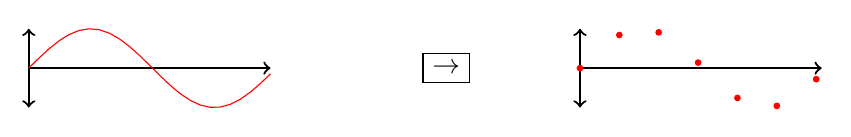
\begin{tikzpicture}[domain =0:6.14, scale = 0.5]
\draw[thick,color=black, ->] (0,0)-- (6.14,0);
\draw[thick, color=black, <->] (0,-1) -- (0,1);
\draw [red] plot  (\x,{sin(\x r)});

\draw[thick,color=black, ->] (14,0)-- (14+6.14,0);
\draw[thick, color=black, <->] (14,-1) -- (14,1);
%\filldraw circle (6,0) (2 pt);
\foreach \i in {1,...,7}{
\pgfmathsetmacro{\y}{sin((\i-1) r)}

\filldraw[red] (14+\i-1,\y) circle (2 pt);

}
\node[draw, rectangle, anchor = west] at (10,0) {$\Large \rightarrow$};
\end{tikzpicture}


\end{block}


\begin{block}{Then to a speaker}
\begin{tikzpicture}[domain =0:6.14, scale = 0.5]
\draw[thick,color=black, ->] (0,0)-- (6.14,0);
\draw[thick, color=black, <->] (0,-1) -- (0,1);
\foreach \i in {1,...,7}{
\pgfmathsetmacro{\y}{sin((\i-1) r)}

\filldraw[red] (\i-1,\y) circle (2 pt);

}
\node[draw, rectangle, anchor = west] at (10,0) {$\Large \rightarrow$};
\node[anchor = west] at (14,0) {\includegraphics[width = 0.25\textwidth]{speaker.png}};
\end{tikzpicture}


\end{block}
\end{frame}


\begin{frame}
\frametitle{How Can 2 Sound Waves Interact?}
\begin{block}{First, what happens when two sound waves meet?}
They add.
\end{block}

\end{frame}

\begin{frame}
\frametitle{The math of 2 wave friends}
\begin{block}{Wave$_1$ \& Wave$_2$}
Suppose Wave$_1 = A\cos(wt + k)$ and Wave$_2 = A\cos(w't + k')$. Then,
\begin{align*}
W_1 + W_2 =&A\cos(wt + k) + A\cos(w't + k')\\
=&2A\cos(\frac{(w+w')t+(k+k')}{2})\cos(\frac{(w-w')t +(k- k')}{2})
\end{align*}
\end{block}

\end{frame}

\begin{frame}
\frametitle{Aural Beating}
\begin{block}{The math of the given example}
Suppose Wave$_1 = \cos(440t)$ and Wave$_2 = \cos(435t)$. Then,
\begin{align*}
W_1 + W_2 =&\cos(440t) + \cos(435t)\\
=&2\cos(\frac{875t}{2})\cos(\frac{5t}{2})
\end{align*}
\end{block}

\begin{block}{}
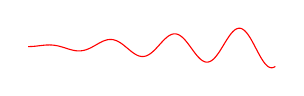
\begin{tikzpicture}[domain =0:3.14, scale = 1, samples = 1000]
\draw [red] plot  (\x,{2*sin( 437.5*\x )*sin(2.5*\x)});
\end{tikzpicture}
\end{block}


\end{frame}

\begin{frame}
\frametitle{Computer Generation of Sound}
\begin{block}{What is Sound on a computer?}

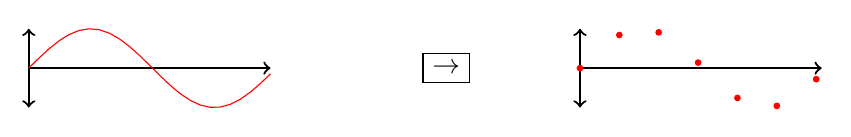
\begin{tikzpicture}[domain =0:6.14, scale = 0.5]
\draw[thick,color=black, ->] (0,0)-- (6.14,0);
\draw[thick, color=black, <->] (0,-1) -- (0,1);
\draw [red] plot  (\x,{sin(\x r)});

\draw[thick,color=black, ->] (14,0)-- (14+6.14,0);
\draw[thick, color=black, <->] (14,-1) -- (14,1);
%\filldraw circle (6,0) (2 pt);
\foreach \i in {1,...,7}{
\pgfmathsetmacro{\y}{sin((\i-1) r)}

\filldraw[red] (14+\i-1,\y) circle (2 pt);

}
\node[draw, rectangle, anchor = west] at (10,0) {$\Large \rightarrow$};
\end{tikzpicture}


\end{block}


\begin{block}{Then to a speaker}
\begin{tikzpicture}[domain =0:6.14, scale = 0.5]
\draw[thick,color=black, ->] (0,0)-- (6.14,0);
\draw[thick, color=black, <->] (0,-1) -- (0,1);
\foreach \i in {1,...,7}{
\pgfmathsetmacro{\y}{sin((\i-1) r)}

\filldraw[red] (\i-1,\y) circle (2 pt);

}
\node[draw, rectangle, anchor = west] at (10,0) {$\Large \rightarrow$};
\node[anchor = west] at (14,0) {\includegraphics[width = 0.25\textwidth]{speaker.png}};
\end{tikzpicture}


\end{block}
\end{frame}

\begin{frame}
\frametitle{How to choose the sampling rate}
\begin{block}{Sampling rate = discretization}
That is to say, the sampling rate has the same issues as discretization choices do in numerical mathematics. How can the necessary information be captured most efficiently?
\end{block}

\begin{block}{CDs}
CDs use 44.1 kHz sampling. Why?
\end{block}
\end{frame}

\begin{frame}
\frametitle{Capturing a pressure wave}
\begin{block}{Sampling at 1.75 of the period}
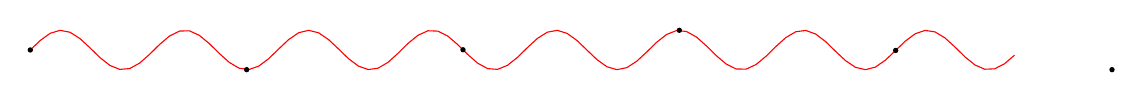
\begin{tikzpicture}[domain =0:50, scale = 0.25, samples = 100]
\draw [red] plot  (\x,{sin(\x r)});
\foreach \i in {1,...,6}{
\pgfmathsetmacro{\x}{3.14*2*(1.75)*(\i-1)}
\pgfmathsetmacro{\y}{sin(\x r)}
\filldraw[black] (\x,\y) circle (3 pt);
}
\end{tikzpicture}
\end{block}

\begin{block}{Sampling at 0.75 of the period}
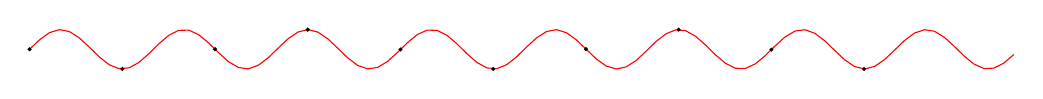
\begin{tikzpicture}[domain =0:50, scale = 0.25, samples = 100]
\draw [red] plot  (\x,{sin(\x r)});
\foreach \i in {1,...,10}{
\pgfmathsetmacro{\x}{3.14*2*(0.75)*(\i-1)}
\pgfmathsetmacro{\y}{sin(\x r)}
\filldraw[black] (\x,\y) circle (2 pt);
}
\end{tikzpicture}
\end{block}

\begin{block}{Sampling at 0.45 of the period}
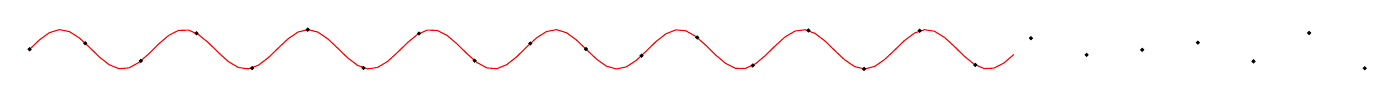
\begin{tikzpicture}[domain =0:50, scale = 0.25, samples = 100]
\draw [red] plot  (\x,{sin(\x r)});
\foreach \i in {1,...,25}{
\pgfmathsetmacro{\x}{3.14*2*(0.45)*(\i-1)}
\pgfmathsetmacro{\y}{sin(\x r)}
\filldraw[black] (\x,\y) circle (2 pt);
}
\end{tikzpicture}
\end{block}
\end{frame}

\begin{frame}
\frametitle{Nyquist Proof}

\begin{block}{Nyquist-Shannon Theorem}
If a function $Q$ is composed of continuous periodic waves (i.e. a nice fourier series) and has a highest frequency component in hertz  $f_{max}$ then the data of a sampling rate of at least $2f_{max}$ can be used to exactly determing $Q$.
\end{block}

\end{frame}

\begin{frame}
\frametitle{Formally...}

\begin{block}{Nyquist-Shannon Theorem}
If a function $Q$ is composed of continuous periodic waves (i.e. a nice fourier series) and has a highest frequency component in hertz  $f_{max}$ then the data of a sampling rate of at least $2f_{max}$ can be used to exactly determing $Q$.
\end{block}

\end{frame}

\begin{frame}
\frametitle{Sounds from instruments}

\begin{block}{Fundamental and overtones}
\center \includegraphics[scale = 0.75]{Harmonics.png};
\end{block}

\end{frame}

\end{document} 